\section{Introduction}
An essential part of parasitic transmission and the evolution of host-pathogen
interactions is the mode of transmission.
Vertical transmission is the direct transfer of a parasite from one generation
to the next during reproduction.
Horizontal transmission is the transmission of parasites among related and
non-related individuals alike, and can be passed on at any time in the hosts’
life cycle\supercite{Ebert:2013}.
Horizontal transmission can occur directly, such as through air-borne,
food-borne or sexual infections, or indirectly through a vector
\supercite{CHEN2006}.
It has been suggested that these different modes of transmission play a crucial
role in determining the virulence of a pathogen
\supercite{Clayton:1994,EWALD:2011}, which reflects its ability to cause
disease\supercite{PAYNE2017}.
The transmission process thus determines the spread and persistence of a given
pathogen in a population, which is crucial to modeling population dynamics and
designing proper disease control strategies.

In 1987, Ewald\supercite{Ewald:1987} theorized that parasites with predominantly
horizontal transmission would tend towards higher virulence, whereas those with
vertical transmission would tend towards lower virulence.
However, Lipsitch et al. (1996)\supercite{Lipsitch:1996} observed that increased
horizontal transmission actually selects for lower virulence and greater vertical
transmission in pathogens instead.
This occurs because of epidemiological feedback: higher contact rates between
hosts allow for a greater number of equilibrium states to be attained, where
high horizontal transmission is not effective\supercite{Lipsitch:1995}.
This enables strains with lower basic reproductive ratios and vertical
transmission to exclude, through competition, those with higher reproductive
ratios and horizontal transmission.

In this study, we successfully replicate the epidemiological model incorporating
trade-offs between vertical and horizontal transmission from the original study
by Lipsitch et al. (1996)\supercite{Lipsitch:1996} using their methods and
parameters.
This study is foundational in the field of evolutionary epidemiology, in that
it challenged the notion that vertical transmission only was able to lower the
evolutionarily stable (ESS) level of virulence, which was the dominant paradigm
at the time.
We observe the dynamics between 1 host population and 100 infected strains added
individually every $10^3$ time steps for a total of $10^5$ iterations.
This model gives the host population time to stabilize and adapt to the exposure
to various pathogens between each transmission opportunity.
Different simulations support the idea that vertical transmission is favoured
over horizontal transmission in cases of decreased virulence, thus selecting
for strains with low virulence.
Furthermore, we find that as the number of opportunities for horizontal
transmission increase, selection for strains with lower virulence also increases,
given that infection is only allowed for one pathogenic strain at a time.
Lastly, we present additional simulations in which each strain’s properties may
evolve through time, thus imitating further realistic conditions.
This study was conducted using version 1.6.0 of the Julia programming language.

\section{Mathematical Model for the Evolution of Virulence}

We start by considering a model composed of one uninfected host population and
two populations infected with either of two pathogenic strains. This model is a
generalization of Lipsitch et al. (1996)\supercite{Lipsitch:1996} single-strain
model and its dynamics are governed by the following equations:

\begin{equation}
\frac{dX}{dt} = (b_x X + e_1 Y_1 + e_2 Y_2)(1 - \frac{X + Y_1 + Y_2}{K}) - u_x X - c X(\beta_1 Y_1 + \beta_2 Y_2)
\label{eqn:1}
\end{equation}

\begin{equation}
\frac{dY_1}{dt} = b_1 Y_1(1 - \frac{X + Y_1 + Y_2}{K}) - u_1 Y_1 + c\beta_1 X Y_1
\label{eqn:2}
\end{equation}

\begin{equation}
\frac{dY_2}{dt} = b_2 Y_2(1 - \frac{X + Y_1 + Y_2}{K}) - u_2 Y_2 + c \beta_2 X Y_2
\label{eqn:3}
\end{equation}

Let $X$ be the number of uninfected hosts and $Y_i$ the number of infected
hosts with pathogen strains $i = 1, 2$. Uninfected hosts have a maximal
\emph{per capita} birth rate $b_x$ and a mortality rate $u_x$, resulting in a
lifespan of $(\frac{1}{u_x})$. Let $e_i$ represent the \emph{per capita} birth
rate of uninfected hosts by hosts infected with strain $i$ and $b_i$ represent
the \emph{per capita} birth rate of offspring infected with strain $i$ per unit
time. Infected hosts die at the rate $u_i \geq u_x$. Let $c$ be the rate of
contact between hosts (i.e. the opportunities for horizontal transmission) and
$\beta_i$ the rate of horizontal transmission of strain $i$. Finally, let $K$
represent the environment’s carrying capacity.

For each strain to invade and persist in the population, the basic reproductive
rate of the parasite must be greater than 1 and satisfy the following conditions:

\begin{equation}
R_0 = H_0 + V_0 > 1
\label{eqn:4}
\end{equation}

\begin{equation}
H_0 = \frac{c \beta_i}{u_i} K(1- \frac{u_x}{b_x})
\label{eqn:5}
\end{equation}

\begin{equation}
V_0 = \frac{b_i u_x}{b_x u_i}
\label{eqn:6}
\end{equation}

Where $H_0$ represents the number of new horizontally-acquired cases from a
single infected host in a population of uninfected hosts before the primary
host dies and $V_0$ represents the number of new vertically-acquired cases by
the same host introduced into the uninfected population at equilibrium.

Generalizing this two-pathogen model to $i$ strains allows for the study of
more complex dynamics, such as in this epidemiological model replication.


\subsection{Justification of Parameters}

Most parameters used in this study are identical to those in the original study.
The initial number of uninfected and infected hosts with strain 1 are of
$X_0$ = 80 and $Y\mysubscript{1.0}$ = 1, respectively. We inferred the former
from the figures in the original article, since this value was not explicitly
mentioned in the text. For the host population, its birth rate $b_x$ is held
constant at 1.0, while its mortality rate $u_x$ is held constant at 0.2.

For plotting purposes, we set the carrying capacity $K$ = 100 to simulate whole
numbers instead of proportions for panels (a,b) of our figures. Also, the values
presented in Figures 1-3 comprise of weighted values for $R_0$, $V_0$, $u_x$,
$\beta_i$ and virulence for noise reduction. We set the value of $K$ = 1 in
panels (c,d) to simplify the calculation of $R_0$. Finally, we plot the evenness
of the total population in panels (i,j) of each figure in order to relate it to
the evolutionary dynamics of each simulation.

The values for variables $c$, $b_i$, $e_i$ and $u_i$ vary between strains and
figures in order to compare their different impacts on the epidemiological
evolutionary trajectories. The horizontal transmission rate and virulence of
each strain are respectively constrained by the following equations:

\begin{equation}
\beta_i(u_i) = \frac{3(u_i - u_x)}{u_i - u_x + 1}
\label{eqn:7}
\end{equation}

\begin{equation}
Virulence = 1 - \frac{(b_i + e_i)u_x}{b_x u_i}
\label{eqn:8}
\end{equation}

Equation (\ref{eqn:7}) defines the monotonically increasing relationship
between disease-induced mortality rates $u_i$ - $u_x$ and horizontal
transmissibility. On the other hand, equation (\ref{eqn:8}) defines virulence
(ranging from 0 to 1) as the proportional fitness loss of an infected host,
where lower virulence equates lower mean mortality.

\subsection{Figure 1}

We compare the evolutionary trajectories with the variable $b_i$ held constant
at the values of 0.1 and 1.0 for every pathogenic strain (thereby calling it a
generalized $b_y$) in their respective column. Since the number of infected
offspring from an infected host $e_i$ directly depends on $b_i$ through the
equation $e_i = b_x - b_i$, each strain also possesses an $e_i$ value of 0.9
and 0.0, in each respective case.

\floatsetup[figure]{style=plain,subcapbesideposition=top}
\begin{figure}[tbph]
    \centering
        \sidesubfloat[a]{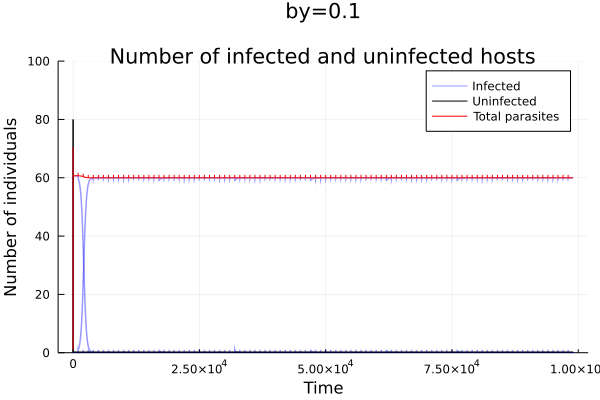
\includegraphics[width=0.4\textwidth]{figures/graph_1a.png}\label{fig:1a}}
    \hfil
        \sidesubfloat[b]{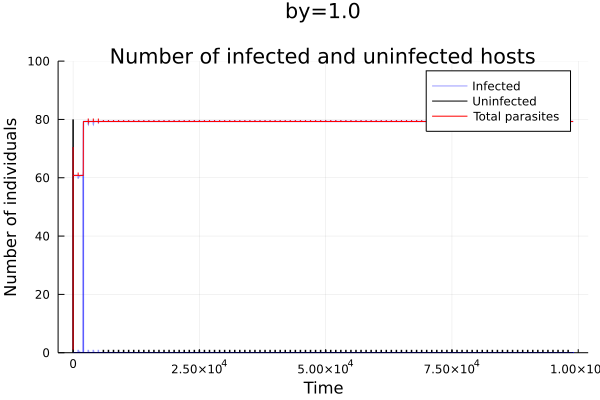
\includegraphics[width=0.4\textwidth]{figures/graph_1b.png}\label{fig:1b}}

    \medskip
        \sidesubfloat[c]{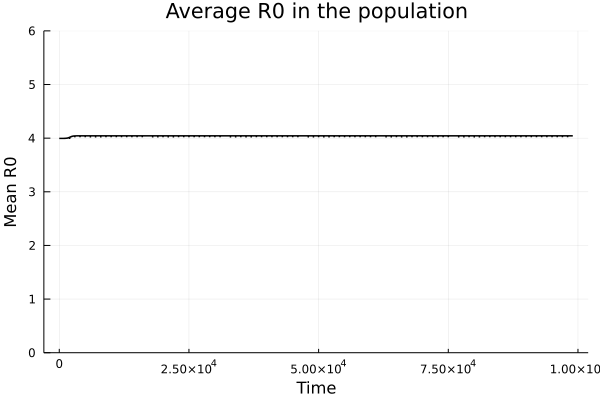
\includegraphics[width=0.4\textwidth]{figures/graph_1c.png}\label{fig:1c}}
    \hfil
        \sidesubfloat[d]{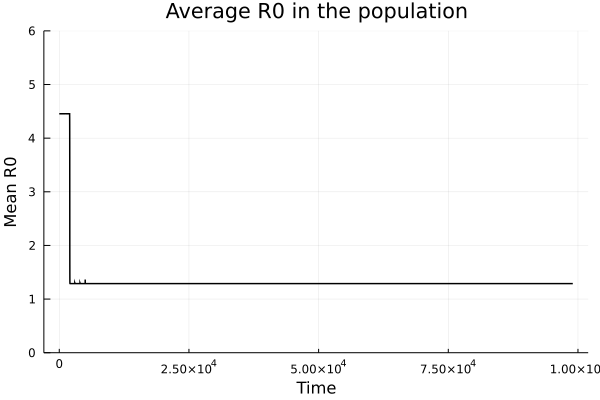
\includegraphics[width=0.4\textwidth]{figures/graph_1d.png}\label{fig:1d}}

    \medskip
        \sidesubfloat[e]{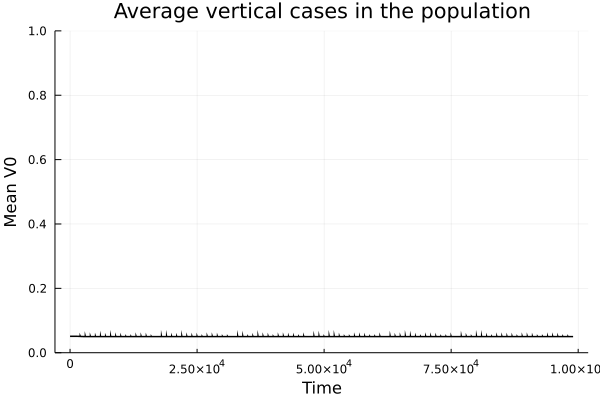
\includegraphics[width=0.4\textwidth]{figures/graph_1e.png}\label{fig:1e}}
    \hfil
        \sidesubfloat[f]{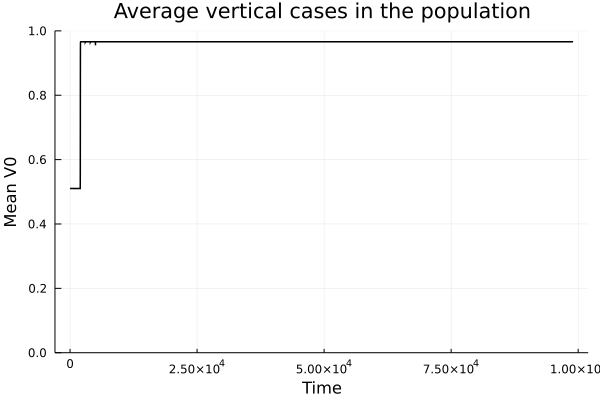
\includegraphics[width=0.4\textwidth]{figures/graph_1f.png}\label{fig:1f}}

    \medskip
        \sidesubfloat[g]{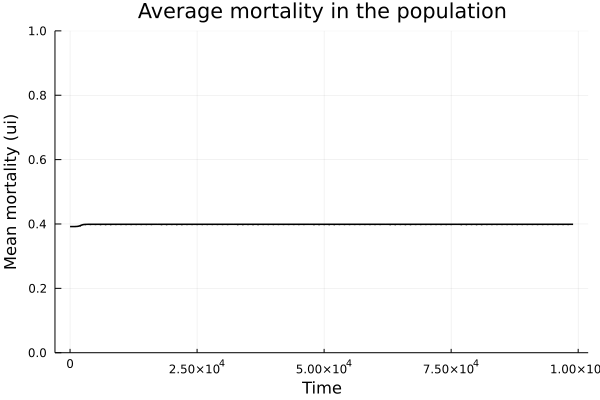
\includegraphics[width=0.4\textwidth]{figures/graph_1g.png}\label{fig:1g}}
    \hfil
        \sidesubfloat[h]{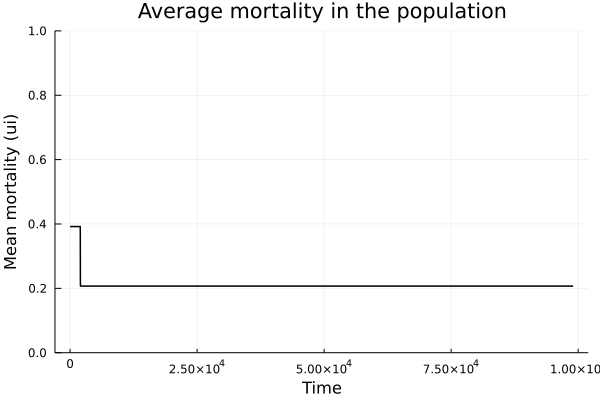
\includegraphics[width=0.4\textwidth]{figures/graph_1h.png}\label{fig:1h}}

    \medskip
        \sidesubfloat[i]{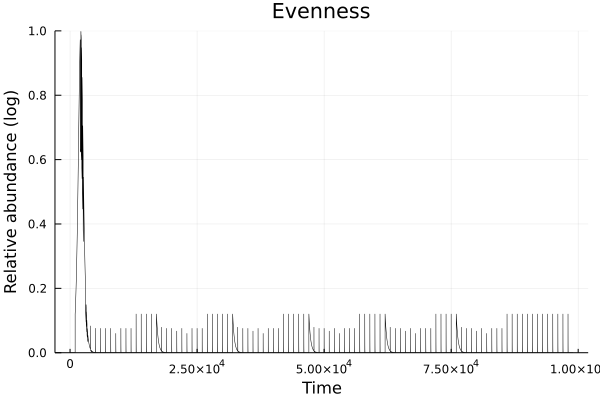
\includegraphics[width=0.4\textwidth]{figures/graph_1i.png}\label{fig:1i}}
    \hfil
        \sidesubfloat[j]{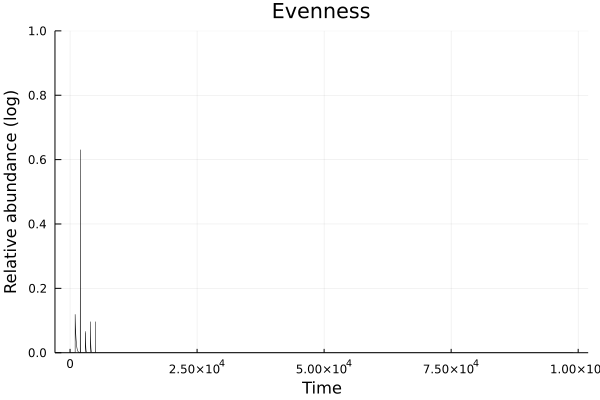
\includegraphics[width=0.4\textwidth]{figures/graph_1j.png}\label{fig:1j}}
\caption{\textbf{Evolutionary dynamics of 100 infected strains introduced every
$10^3$ generations for two vertical transmission values, $b_i = 0.1$ (left) and
$b_i = 1.0$ (right)}. We demonstrate (a,b) the number of uninfected and infected
hosts with each strain; (c,d) the mean $R_0$ in the population; (e,f) the
average of all new infections acquired vertically; (g,h) the average mortality
in the population; (i,j) the evenness of the total population. We show that
higher vertical transmission selects for lower mortality, horizontal
transmission and $R_0$. Constants: $c = 4.0$, $b_x = 1.0$,
$u_x = 0.2$, $e_i = b_x - b_i$. Each infected strain possesses a random value
of $u_i$ \in [$u_x$, 1] which in turn determines its value of $\beta_i$
according to equation \ref{eqn:7}. \textit{We successfully reproduced Figure 1
from its corresponding figure in the original study. Despite the minor
differences due to the random variable permutations, our results follow the
same trends.}
}
\label{fig:figure1}
\end{figure}

\subsection{Figure 2}

We present the evolutionary trajectories with additional variables $r_1$,
$r_2$ and $r_3$. Their values are randomly sampled on a uniform distribution
over [0,1] for each strain in order to add stochasticity to the model. They
respectively designate the total virulence of the strain, the fraction of
virulence attributable to fecundity loss, and the fraction of offspring of
infected hosts which are infected. The resulting constraints on the simulations’
parameters are the following:

\begin{equation}
e_i = b_x(1 - r_3)(1- r_1 r_2)
\label{eqn:9}
\end{equation}

\begin{equation}
b_i = b_x r_3(1 - r_1 r_2)
\label{eqn:10}
\end{equation}

\begin{equation}
\beta_i = r_1 - \frac{\alpha b_i}{b_x}
\label{eqn:11}
\end{equation}

Equation \ref{eqn:9} mathematically depicts that the birth rate of uninfected
offspring by infected hosts $e_i$ is equal to the maximal \emph{per capita}
birth rate $b_x$ multiplied by the fraction of uninfected offspring (1 - $r_3$)
minus the fecundity loss due to virulence (1 - $r_1$ $r_2$). Equation
\ref{eqn:10} shows that the birth rate of infected offspring $b_i$ is equal to
the maximal \emph{per capita} birth rate $b_x$ multiplied the fraction of
infected offspring $r_3$ minus this same loss. Finally, equation \ref{eqn:11}
reveals that the rate of horizontal transmission $\beta_i$ is equal to the
total virulence $r_1$ minus the cost of vertical transmission in relation to
horizontal transmission $\alpha$ multiplied by the fraction of infected births
$b_i$/$b_x$. We set the parameter $\alpha$ as a random value over [0,1] for each
strain, introducing a cost-benefit trade-off between vertical and horizontal
modes of transmission on parasite fitness. We ensure non-negative horizontal
transmission values by setting $\beta_i$ to zero if the second term happens to
be greater than the first term by chance.

\begin{figure}[tbp]
    \centering
        \sidesubfloat[a]{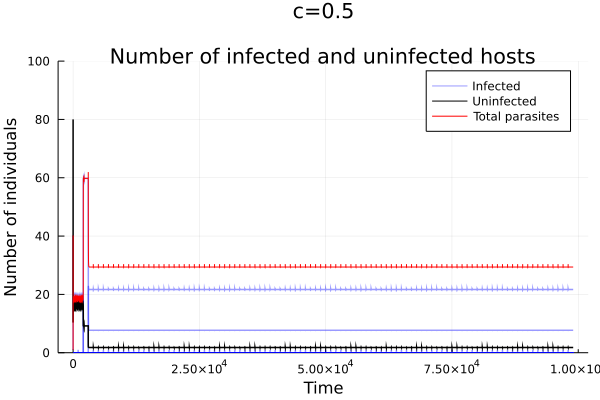
\includegraphics[width=0.4\textwidth]{figures/graph_2a.png}\label{fig:2a}}
    \hfil
        \sidesubfloat[b]{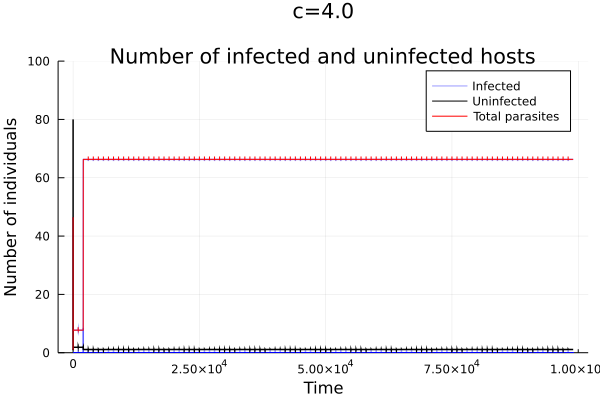
\includegraphics[width=0.4\textwidth]{figures/graph_2b.png}\label{fig:2b}}

    \medskip
        \sidesubfloat[c]{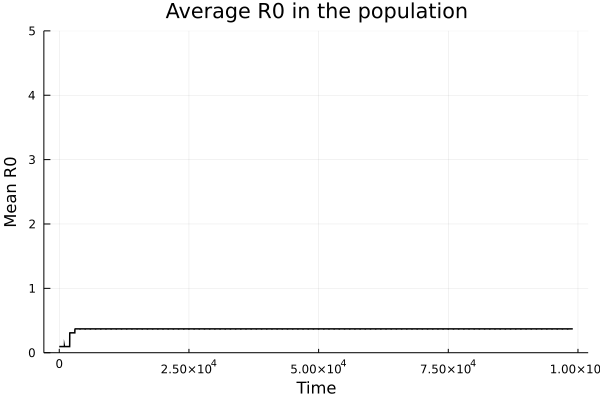
\includegraphics[width=0.4\textwidth]{figures/graph_2c.png}\label{fig:2c}}
    \hfil
        \sidesubfloat[d]{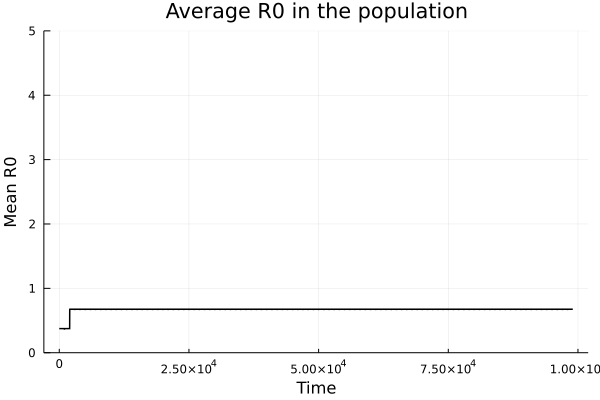
\includegraphics[width=0.4\textwidth]{figures/graph_2d.png}\label{fig:2d}}

    \medskip
        \sidesubfloat[e]{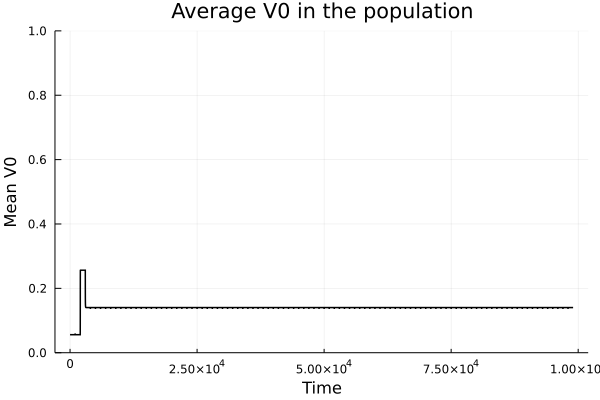
\includegraphics[width=0.4\textwidth]{figures/graph_2e.png}\label{fig:2e}}
    \hfil
        \sidesubfloat[f]{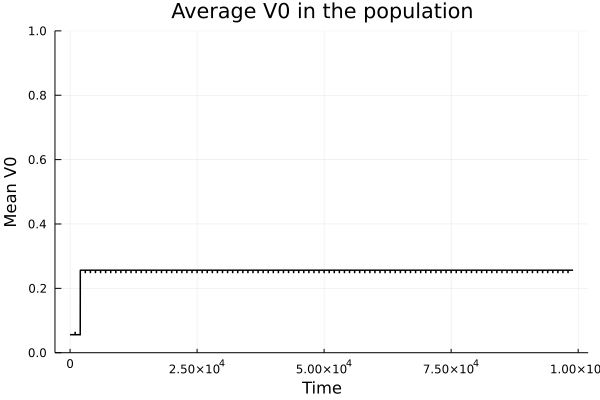
\includegraphics[width=0.4\textwidth]{figures/graph_2f.png}\label{fig:2f}}

    \medskip
        \sidesubfloat[g]{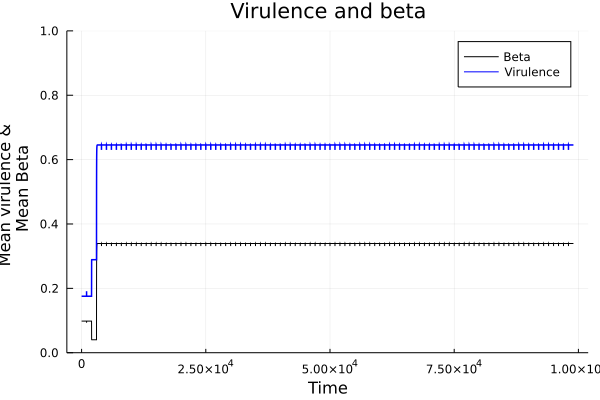
\includegraphics[width=0.4\textwidth]{figures/graph_2g.png}\label{fig:2g}}
    \hfil
        \sidesubfloat[h]{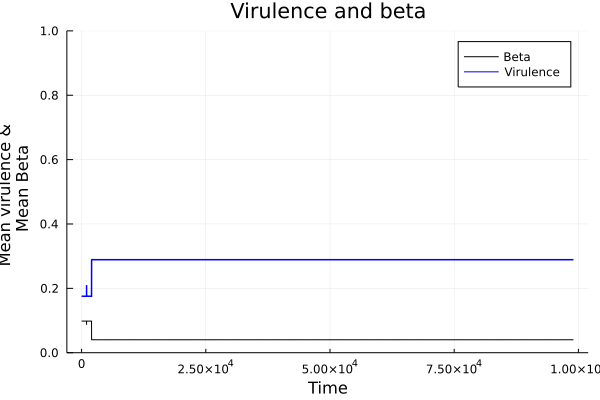
\includegraphics[width=0.4\textwidth]{figures/graph_2h.png}\label{fig:2h}}

    \medskip
        \sidesubfloat[i]{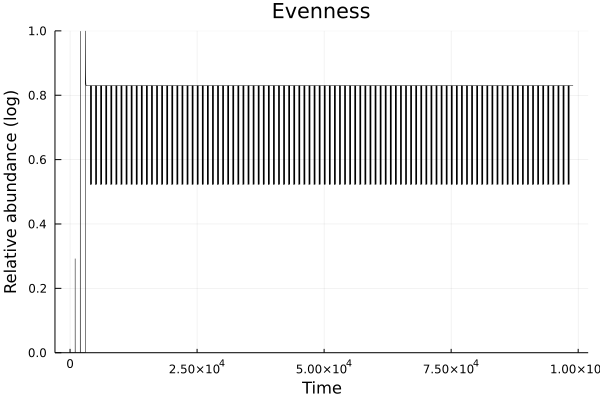
\includegraphics[width=0.4\textwidth]{figures/graph_2i.png}\label{fig:2i}}
    \hfil
        \sidesubfloat[j]{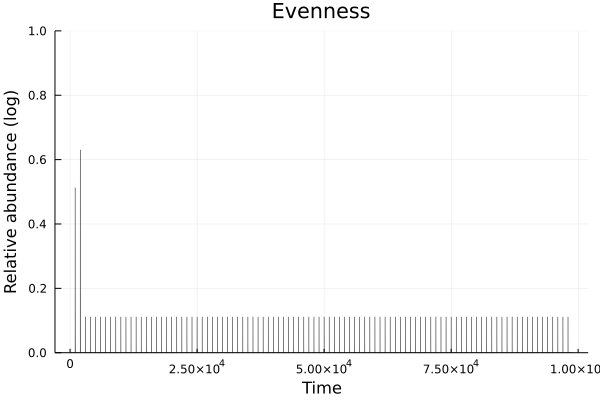
\includegraphics[width=0.4\textwidth]{figures/graph_2j.png}\label{fig:2j}}
\caption{\textbf{Evolutionary dynamics of 100 infected strains introduced every
$10^3$ generations for two horizontal transmission opportunity, $c = 0.5$ (left)
and $c = 4.0$ (right).} The parameters are identical to those in Figure 1 but
with $e_i$, $b_i$ and $\beta_i$ constrained through equations (\ref{eqn:9}),
(\ref{eqn:10}) and (\ref{eqn:11}). We demonstrate (a,b) the number of uninfected
and infected hosts with each strain; (c,d) the mean $R_0$ in the population;
(e,f) the average of all new infections acquired vertically; (g,h) the average
virulence and horizontal transmission rate $\beta_i$; (i,j) the evenness of the
total population. We show that a higher contact rate $c$ selects for lower
virulence at equilibrium and higher vertical transmission rates. The variability
induced by the parameters here allow for strains of high vertical transmission
and low virulence to persist. Constants: $b_x = 1.0$ and $u_x = 0.2$. Each
infected strain possesses a random value of $u_i$ \in [$u_x$, 1].
\textit{We successfully reproduced Figure 2 from its corresponding figure in the
original study. Although our results follow the same trends, our simulations
demonstrate lower values of $V_0$, virulence and $\beta_i$, on top of minor
differences due to stochasticity.}
}
\label{fig:figure2}
\end{figure}

\subsection{Figure 3}

We show the evolutionary trajectories where both vertical and horizontal
transmission parameters can vary with a constraint. All parameters are identical
to those in Figure 2, with the exception of $r_3$ restricted by the range
[0, $r_1$] such that the fraction of infected offspring from infected hosts
may not exceed the total virulence.

\begin{figure}[tbp]
    \centering
        \sidesubfloat[a]{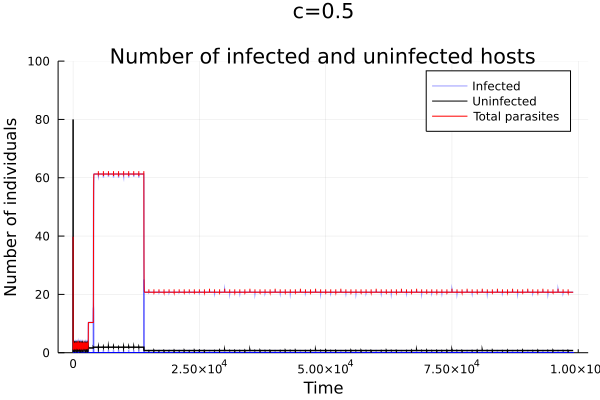
\includegraphics[width=0.4\textwidth]{figures/graph_3a.png}\label{fig:3a}}
    \hfil
        \sidesubfloat[b]{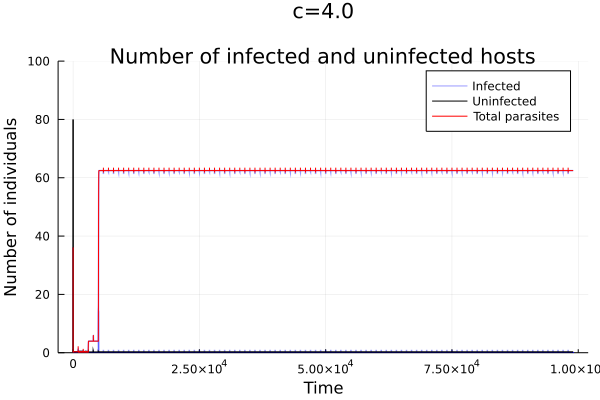
\includegraphics[width=0.4\textwidth]{figures/graph_3b.png}\label{fig:3b}}

    \medskip
        \sidesubfloat[c]{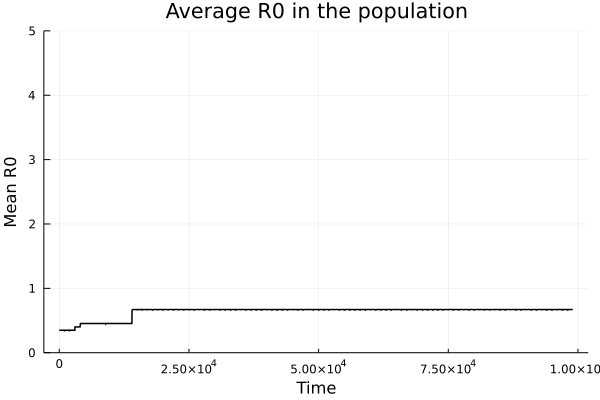
\includegraphics[width=0.4\textwidth]{figures/graph_3c.png}\label{fig:3c}}
    \hfil
        \sidesubfloat[d]{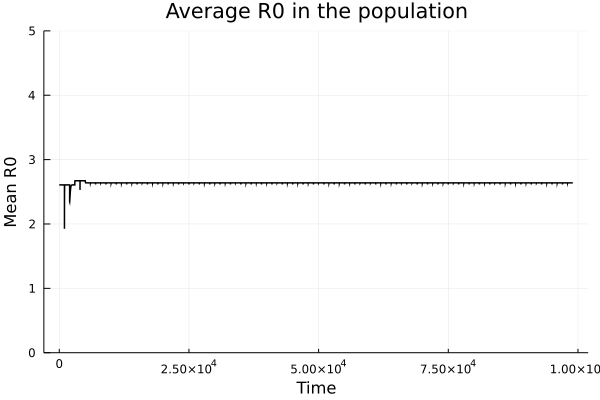
\includegraphics[width=0.4\textwidth]{figures/graph_3d.png}\label{fig:3d}}

    \medskip
        \sidesubfloat[e]{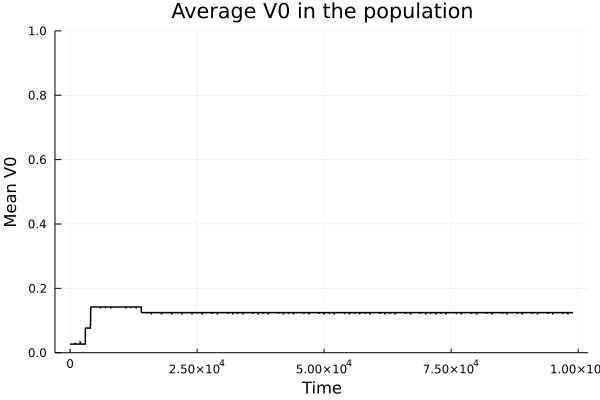
\includegraphics[width=0.4\textwidth]{figures/graph_3e.png}\label{fig:3e}}
    \hfil
        \sidesubfloat[f]{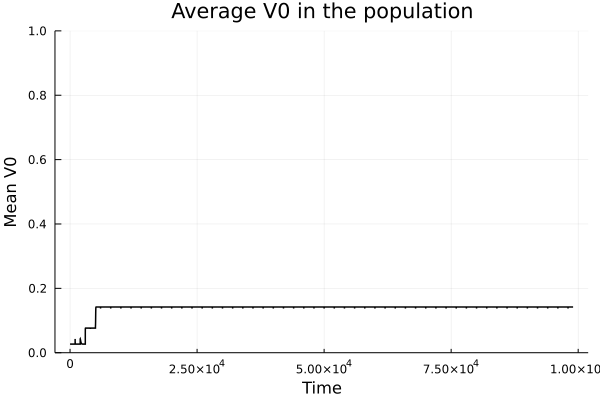
\includegraphics[width=0.4\textwidth]{figures/graph_3f.png}\label{fig:3f}}

    \medskip
        \sidesubfloat[g]{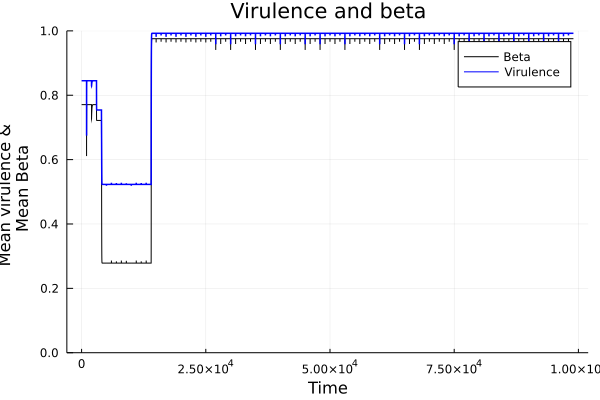
\includegraphics[width=0.4\textwidth]{figures/graph_3g.png}\label{fig:3g}}
    \hfil
        \sidesubfloat[h]{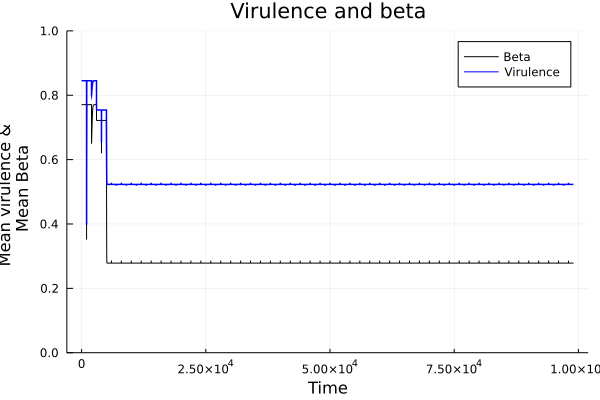
\includegraphics[width=0.4\textwidth]{figures/graph_3h.png}\label{fig:3h}}

    \medskip
        \sidesubfloat[i]{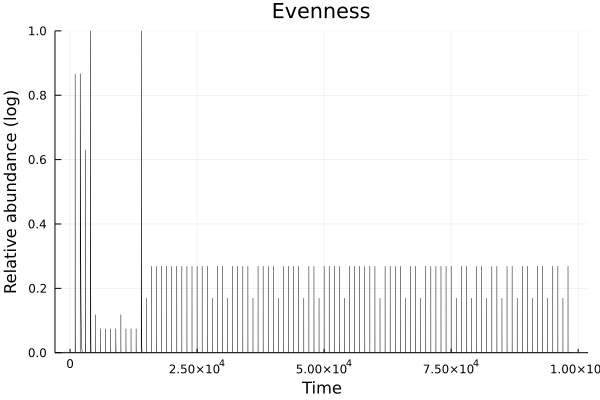
\includegraphics[width=0.4\textwidth]{figures/graph_3i.png}\label{fig:3i}}
    \hfil
        \sidesubfloat[j]{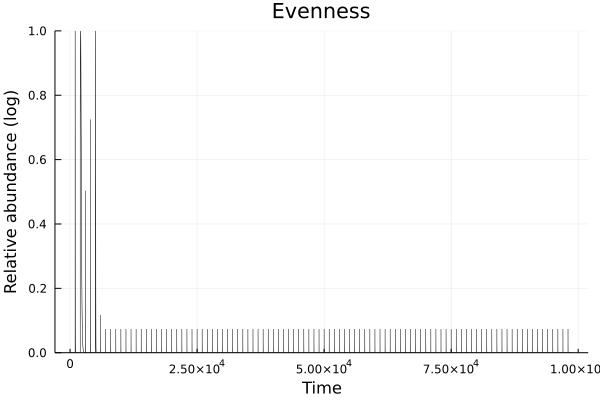
\includegraphics[width=0.4\textwidth]{figures/graph_3j.png}\label{fig:3j}}
\caption{\textbf{Evolutionary dynamics of 100 infected strains introduced every
$10^3$ generations for two values of horizontal transmission opportunity,
$c = 0.5$ (left) and $c = 4.0$ (right).} All parameters are identical to those
in Figure 2 but with a constraint $r_3$ chosen randomly from a uniform
distribution over [0, $r_1$] per strain. We demonstrate (a,b) the number of
uninfected and infected hosts with each strain; (c,d) the mean $R_0$; (e,f) the
average of all new infections acquired vertically; (g,h) the average virulence
and horizontal transmissibility $\beta_i$; (i,j) the evenness of the total
population. Similarly, we show that a higher contact rate $c$ selects for lower
virulence and higher vertical transmission rates. However, higher levels of
virulence evolve and an increase in vertical transmission results in little
fitness benefit. \textit{We successfully reproduced Figure 3 from its
corresponding figure in the original study. Our results follow the same trends,
although our simulations for $c = 4.0$ demonstrate lower values of $R_0$ and
$V_0$.}
}
\label{fig:figure3}
\end{figure}

\section{Discussion}
\subsection{Parameter Constraints}

In Figure \ref{fig:figure1}, we replicate the evolutionary trajectories for
two different values of vertical transmission, $b_y = 0.1$ and $1.0$, which
are held constant for all strains. This scenario represents a case of imperfect
vertical transmission such that there is no net loss of fertility due to
infection. In other words, virulence (i.e. the loss of fitness of the host)
depends solely on mortality through equation (\ref{eqn:8}); we thus neglect
the decrease in fitness from the reduction of the number of uninfected offspring.

In the following two figures, we replicate simulations of the evolutionary
dynamics with varying vertical and horizontal parameters under constraints
through equations (\ref{eqn:9}-\ref{eqn:11}). In Figure \ref{fig:figure2},
strains are permitted to have very low virulence and very high vertical
transmission (through random variables $r_1$, $r_2$, $r_3$ and $\alpha$). This
state is typically seen in the evolution of avirulence. In Figure
\ref{fig:figure3}, high levels of vertical transmission are only permitted with
high levels of virulence through the $r_3$ \in [0, $r_1$] restriction. This is
typically associated with pathogens that require sufficient replication within
the host, usually resulting in the harming of the host.

\subsection{Analysis of Results}
As shown in Figure \ref{fig:figure1}, different parasitic strains persist due
to coexistence and competitive exclusion, which varies in degree at every new
generation. Similarly to the results observed by Lipsitch et al.
(1996)\supercite{Lipsitch:1996}, higher vertical transmission selects for lower
mortality, horizontal transmission and $R_0$. This indicates a lesser importance
of the horizontal transmission parameter, in the case where there is a higher
vertical transmission rate; this represents a situation in which the population
is saturated with individuals infected by pathogens with high vertical
transmission and low virulence. Additionally, lower virulence results in lower
mean mortality through equation \ref{eqn:8} and as observed in panels (g, h).
Panels (i,j) describe the evenness of the total population, which is observed
to remain at low values in both situations. Because of the high reproductive
rate ($R_0 > 1$), a small number of strains occupy the majority of the
population, while close to no hosts remain uninfected.

Figure \ref{fig:figure2} shows the evolutionary trajectories where high vertical
transmission is compatible with low virulence. Two cases with identical
parameters except for the rate of contact between hosts, $c = 0.5$ and
$c = 4.0$, are presented. As predicted in the original study, an increase in the
contact rate selects for less virulent strains exhibiting high vertical
transmission rates. This can be explained by the fact that as the number of
contacts between individuals increases, the number of available susceptible
individuals decreases, leading to saturation.

Figure \ref{fig:figure3} describes an equilibrium similar to that of Figure
\ref{fig:figure2}, but with increases in virulence. This can be explained
through the limit on vertical transmission (through the constraint $r_3$ \in
[0, $r_1$] and the low rate of horizontal transmission, which is directly
correlated to the contact rate ($c = 0.5$). Equation \ref{eqn:4} confirms this
observation, where the invasion and persistence of a parasite can only occur
when the sum of $H_0$ and $V_0$ is greater than 1. Selection thus favours
parasites exhibiting relatively high virulence and employing horizontal
transmission. As previously described, the fraction of infected offspring from
infected hosts, and thus vertical transmission, is limited by the total
virulence of the strain. This constraint results in the mean $V_0$ barely
attaining a vertical basic reproductive ratio of 0.2, thus demonstrating the
limited fitness benefit conferred by vertical transmission. We therefore
confirm the results from Lipsitch et al. (1996)\supercite{Lipsitch:1996}, where
horizontal transmission is less virulent than vertical transmission. Our
simulations show that natural selection will always select for strains of lower
virulence, which explains the decrease in virulence shown in panels (g,h).

In Figures \ref{fig:figure2} and \ref{fig:figure3}, selection for the type of
transmission will depend on whether high vertical transmission is limited by
virulence. When there is a competition between both transmission types, there
will always be selection for the type that guarantees greater host fitness. And
as seen in Ebert and Bull (2003), vertically-transmitted strains are less
virulent than horizontally-transmitted ones. A horizontally-transmitted strain
will always push the host to invest its energy in contact rather than
reproduction, while vertical transmission ensures the opposite. A less virulent
strain using vertical transmission provides the host with greater fitness than a
very virulent strain using horizontal transmission, which therefore guarantees
its persistence in the population over time. This dynamic is reflected in the
relationship between virulence and the type of transmission\supercite{Levin:1996}.
However, in the case where high vertical transmission requires high virulence,
horizontally-transmitted pathogens would prevail because of the low fitness
benefits from vertical transmission.

\subsection{Other Remarks}
In this replication study, we observe fewer variation and trade-offs between
competing strains in panels (a,b) of Figures 1-3, since the infected persist
faster and certain dominant strains take over the entire population for the
remainder of the simulations. We also notice generally lower $R_0$ and $V_0$
values than expected from the simulations in Lipsitch et al. (1996)
\supercite{Lipsitch:1996}. This could be attributed to the variability induced
by the four random variables $r_1$, $r_2$, $r_3$ and $\alpha$ (where the latter
in particular was chosen as a random value over [0,1] per strain due to a lack
of information in the original study) or to potentially different initial
numbers of individuals (which were also arbitrarily chosen due to their values
not being explicitly mentioned in the text). It could also be explained by the
differences in duration of the simulations; this replication was done on a
smaller scale, with ten times less strains, such that the probability of one
random strain overcoming the one with the highest fitness is reduced by a
factor of ten. Finally, we note that the population evenness is inversely
related to the presence of dominant strains; very few strains monopolizing the
population result in low evenness, whereas multiple strains co-existing result
in a population exhibiting higher evenness. Panels (i,j) of each figure depict
the expected dynamics in such cases.

\subsection{Conclusion}
Few models consider the evolution of virulence for parasites with mixed
horizontal and vertical transmission. Here, our results are similar to the
findings of Lipsitch et al. (1996)\supercite{Lipsitch:1996}, suggesting that
selection depends on whether high vertical transmission rates are constrained
by low or high virulence. Similarly, we observed that selection favours
vertically-transmitted strains, but only when vertical transmission is
compatible with low virulence. On the other hand, in situations where high
vertical transmission rates are only possible with high virulence, horizontal
transmission is favoured. Ultimately, selection will always favour the least
virulent strain, regardless of the type of transmission.

These findings could suggest that efforts to reduce vertical transmission of
pathogens could, unintentionally, shift selection towards mutants of increased
virulence. It is possible that vertical transmission has placed a selection
pressure on pathogens to evolve at relatively low levels of virulence, thereby
allowing the mother-to-offspring chain of transmission to continue over several
generations. However, in cases where the horizontal transmission rates are also
low, reducing vertical transmission might be sufficient to eliminate a pathogen
from a population by bringing its basic reproductive ratio below unity.
